\documentclass[../main.tex]{subfiles}

\graphicspath{{\subfix{../images/}}}

\begin{document}

\section{Concepción de la base de datos}

\subsection{Identificación de requerimientos funcionales}

\begin{enumeratedtable}[prefix=F]
  \item{El sistema permite al estudiante matricularse en uno o más cursos de su preferencia.}
  \item{El sistema permite al estudiante obtener uno o más certificados de los cursos aprobados.}
  \item{El sistema permite al usuario retirarse del curso en caso así lo solicite.}
  \item{El sistema permite a las instituciones afiliadas publicar diversos contenidos educativos.}
  \item{El sistema ofrece convenios a las instituciones afiliadas para proveer servicios especializados.}
  \item{El sistema permite a los diversos usuarios interactuar entre sí mediante foros masivos de consulta de un determinado curso.}
  \item{El sistema permite al estudiante acceder a gran cantidad de material audiovisual, lecturas y actividades en un curso.}
  \item{El sistema recomienda cursos al usuario según sus especializaciones previas en determinado ámbito.}
  \item{El sistema permite al usuario referenciar sus logros obtenidos en Linkedin.}
  \item{El sistema permite al usuario cursar programas totalmente gratuitos. Sin embargo, debe pagar si desea obtener el certificado correspondiente.}
\end{enumeratedtable}

\subsection{Hipótesis}

\subsubsection{Sobre el servicio}

El alumno puede inscribirse a los cursos dependiendo de su modalidad.
Se le concederá acceso al módulo correspondiente al curso. Ahí podrá
realizar las actividades, encontrar los documentos y más. Al llegar al
final del curso, tendrá que calificar para recibir el certificado y
agregarse al apartado de logros. De ser así, se le otorgará
dependiendo de la modalidad ya que puede ser de pago.

\subsubsection{Sobre las instituciones}

\begin{enumerate}
  \item Ofrecen cursos con sus docentes a Coursera mediante colaboraciones.
  \item Tienen acceso a los datos de los docentes y alumnos.
\end{enumerate}

\subsubsection{Sobre los instructores}

\begin{enumerate}
  \item Para que el docente pueda ofrecer su curso debe estar calificado
        y pertenecer a una institución.
  \item Podrá acceder a los datos del estudiante inscrito en su curso.
  \item Puede calificar las actividades realizadas por los estudiantes.
\end{enumerate}

\subsubsection{Sobre el estudiante}

El estudiante tendrá un amplio catálogo de cursos separados por categorías
y subcategorías. Puede inscribirse gratuitamente o con un pago mensual,
esto depende del plan del alumno. El estudiante tendrá que cumplir con las
actividades y estudiar el material que el curso ofrezca. Al completar con
éxito sus exámenes, se le calificará si cumple con los requisitos para
acceder al certificado del curso. Este puede ser gratuito o de pago.
En el certificado irá el nombre de la institución, la fecha, los datos
del estudiante y docente, y el curso.

\subsection{Entidades, atributos y sus restricciones}

\subfile{attribute-tables.tex}

\subsection{Modelo de procesos principales de la empresa}

\subsubsection{Proceso de matrícula y certificación}

\begin{figure}[H]
  \centering
  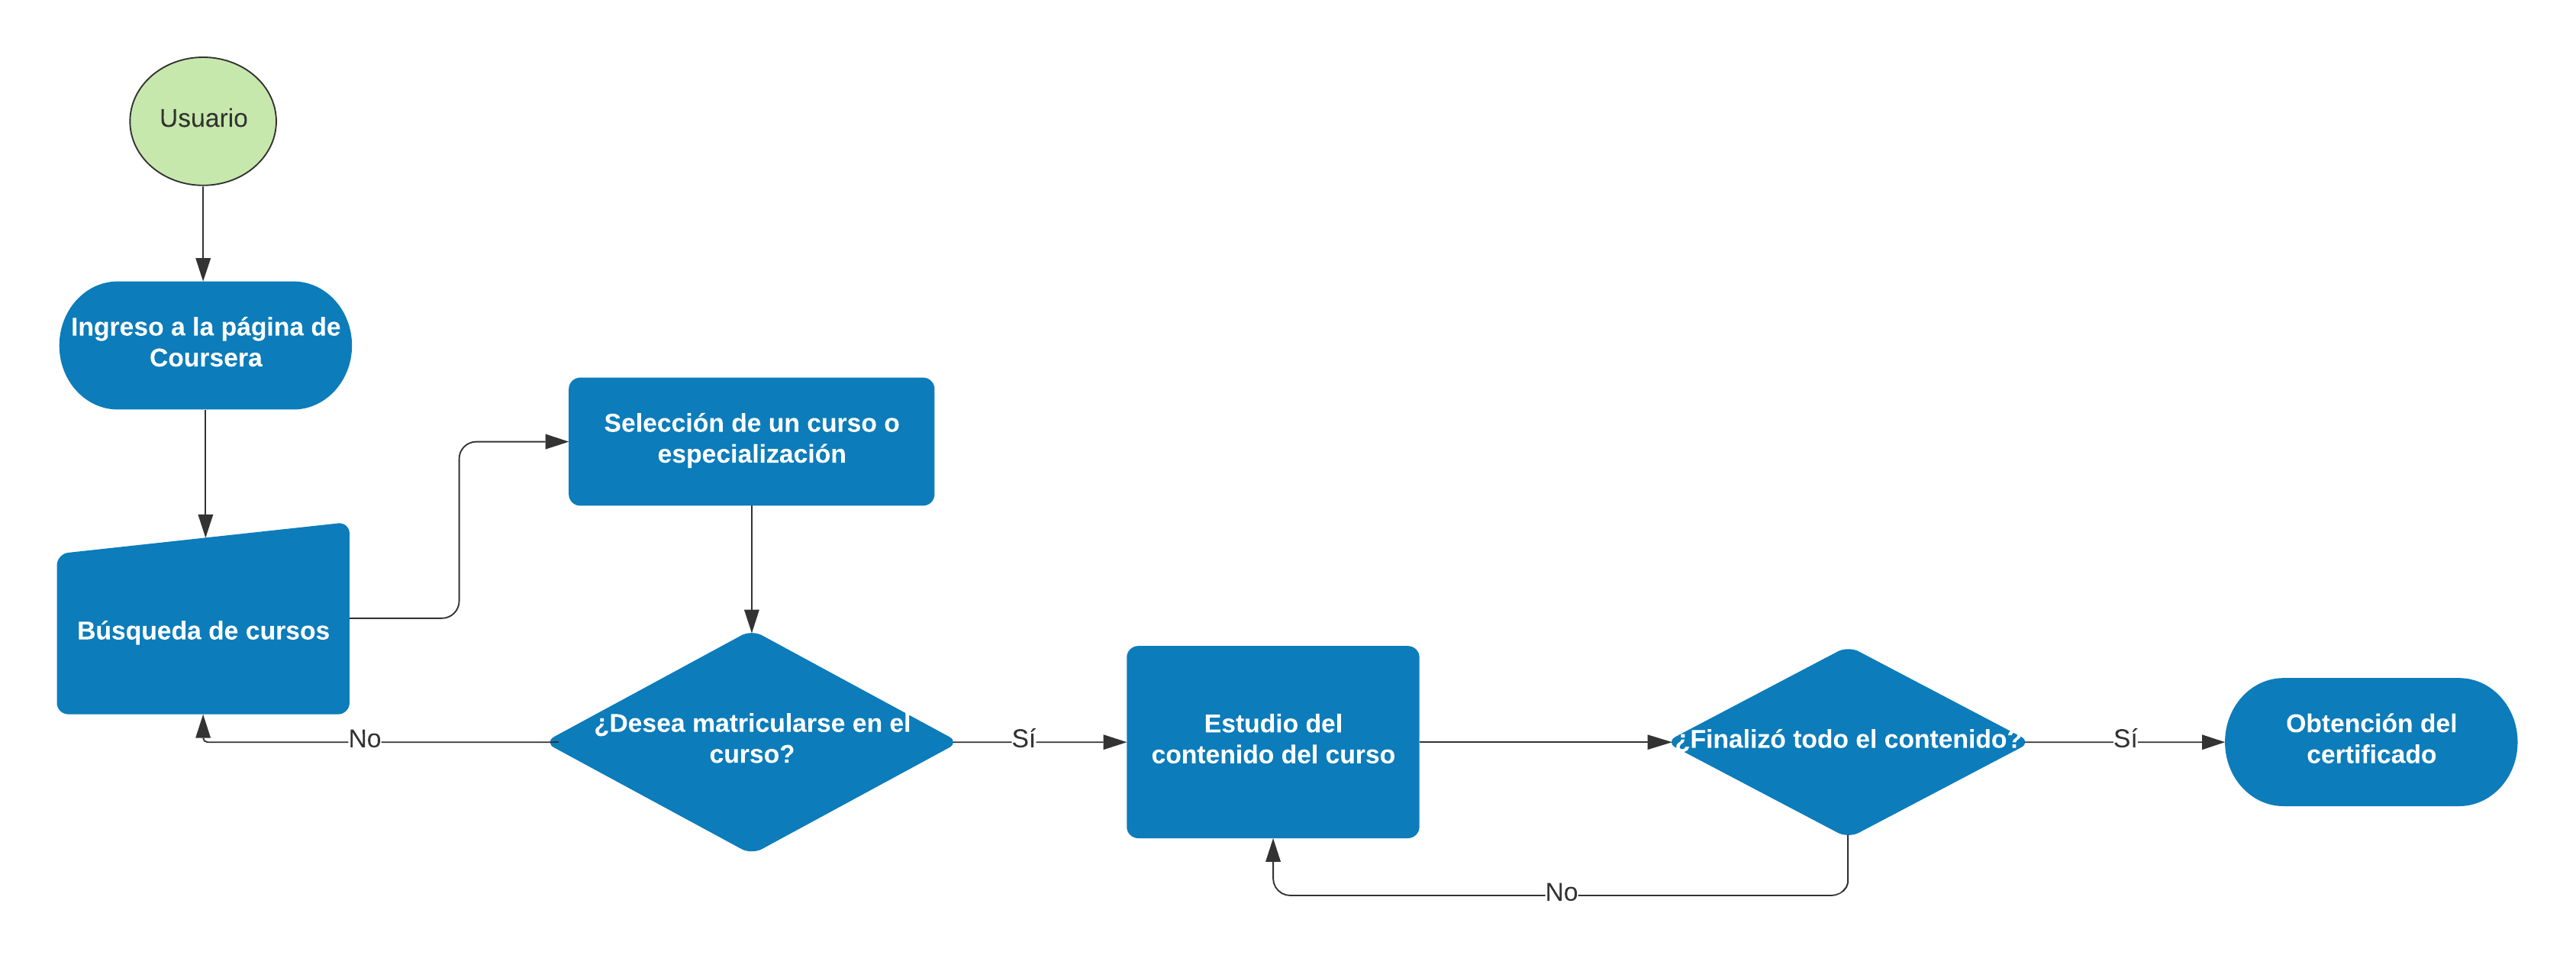
\includegraphics[width=1\linewidth]{procesos-principales}
\end{figure}

\subsection{Diagrama Entidad-Relación}

\begin{figure}[H]
  \centering
  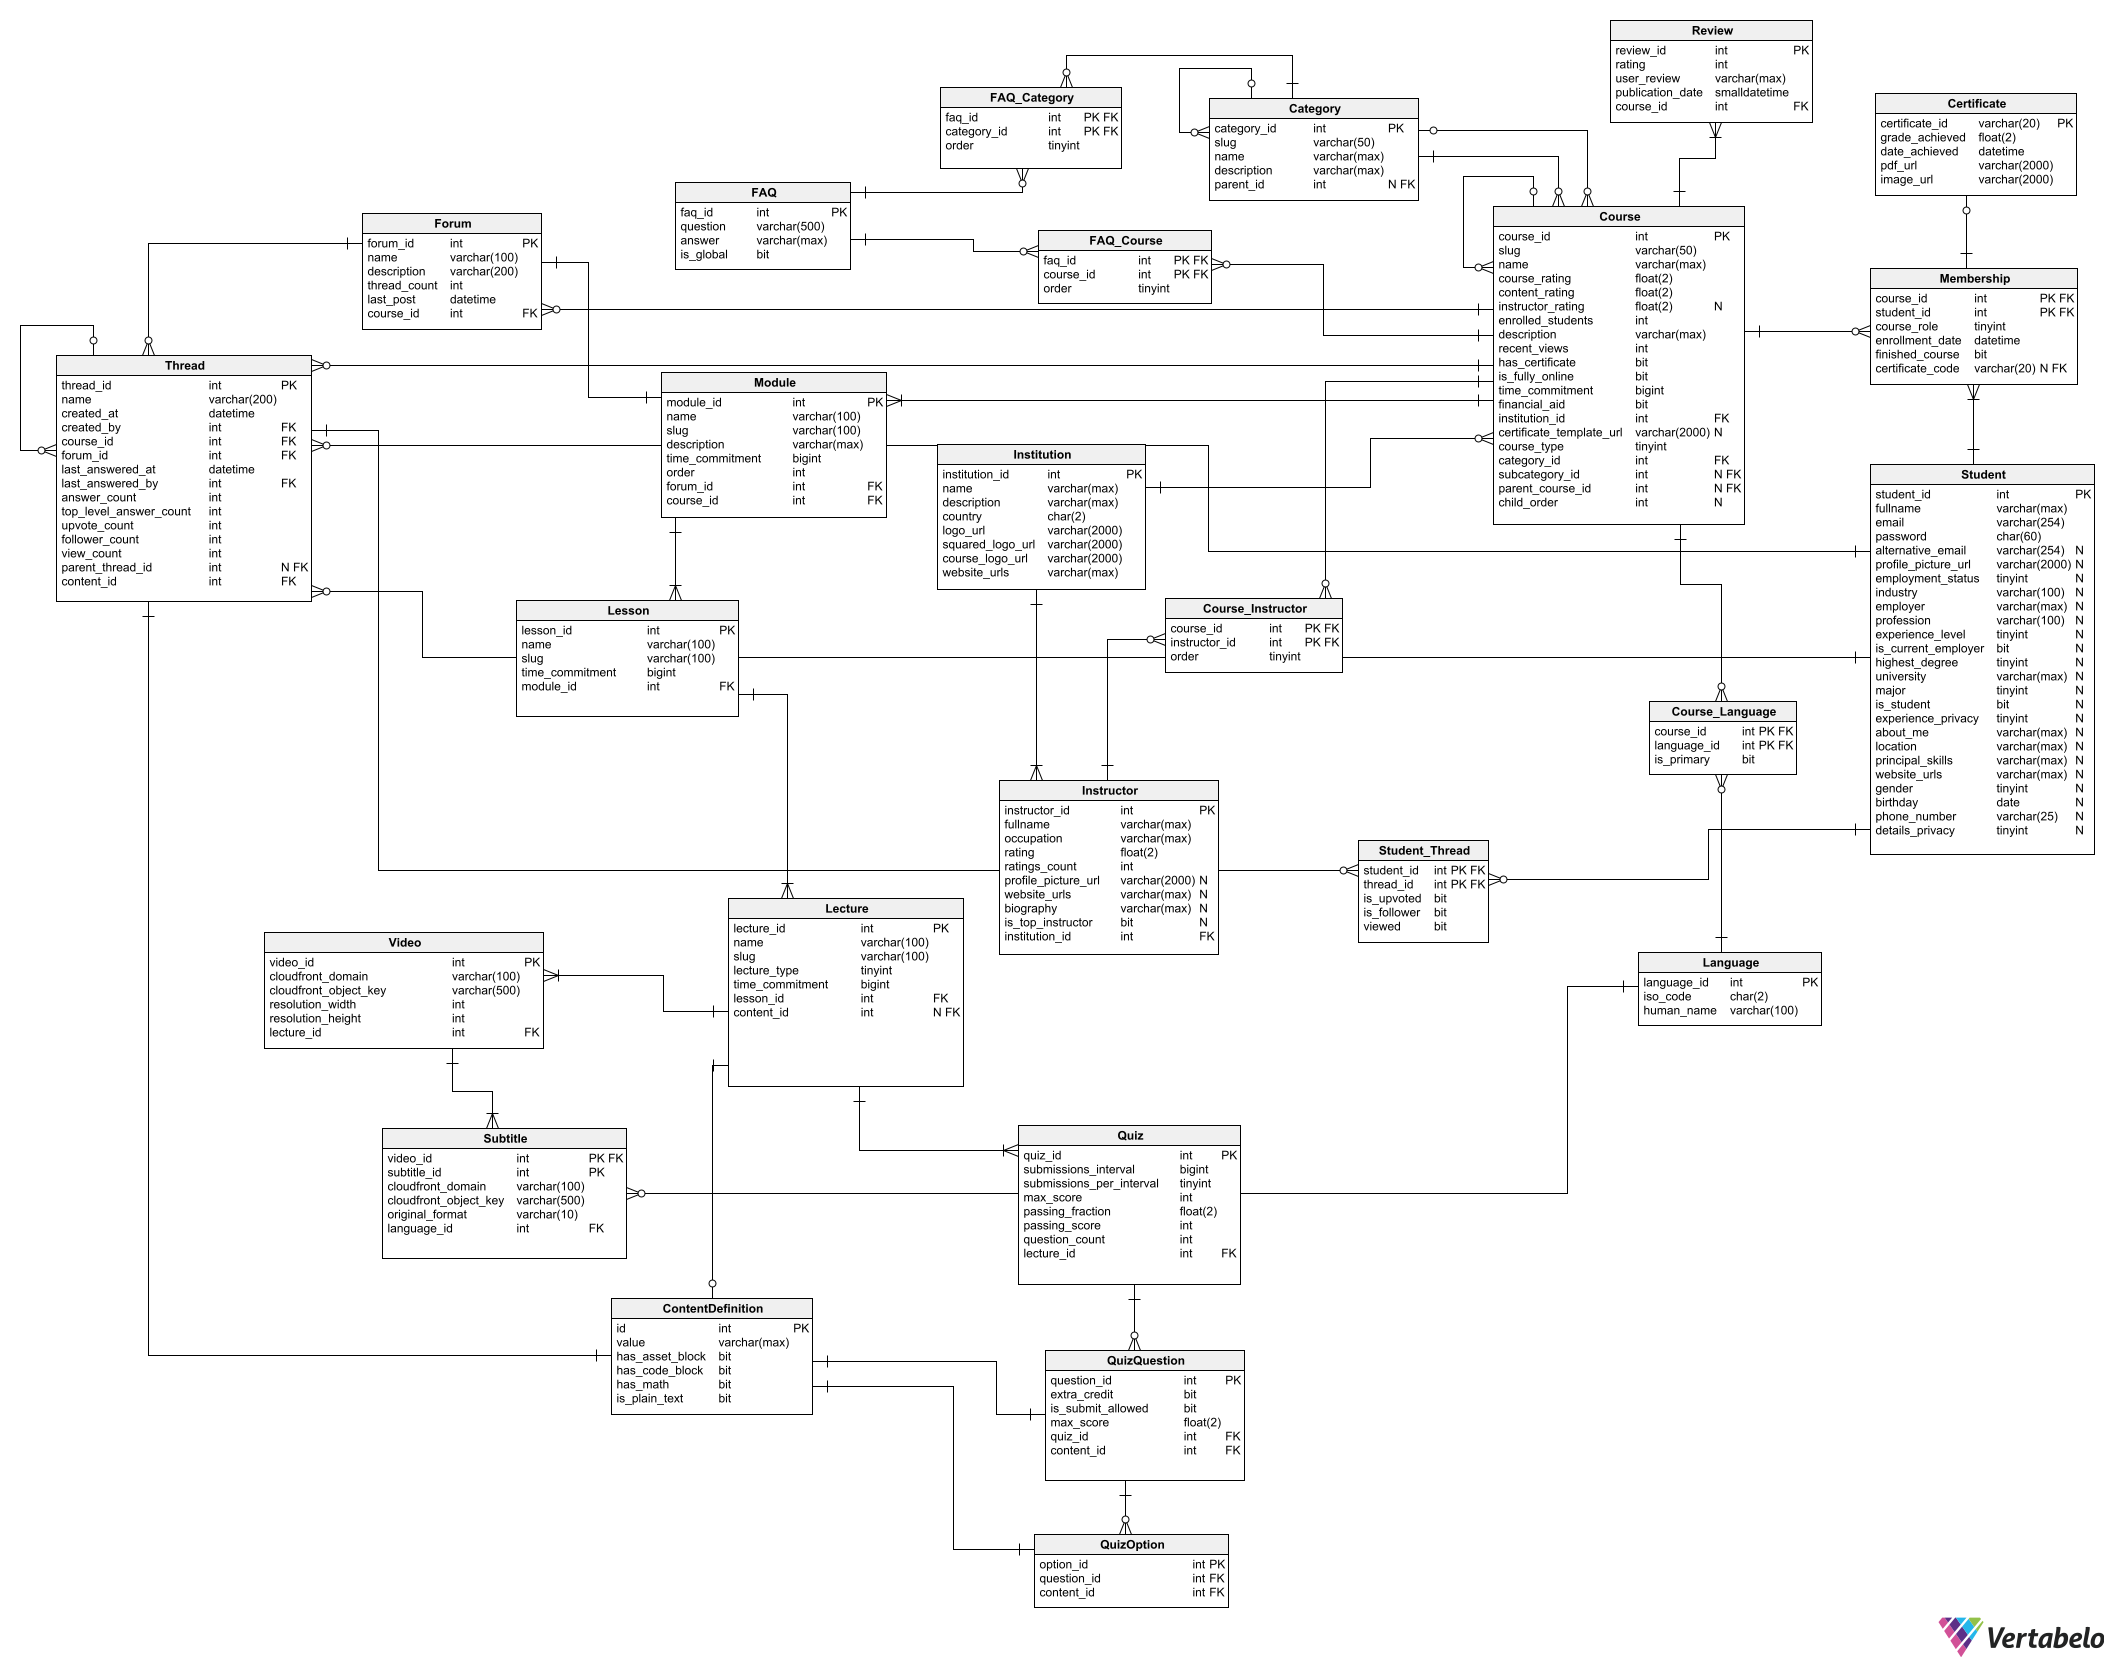
\includegraphics[width=1\linewidth]{database-diagram}
\end{figure}

Versión web disponible en \href{https://my.vertabelo.com/public-model-view/ukHs6uqjUATeSLbRCSPE2cxNynnT7Ih2eVq5pHasMIKzGy4rT7edH539Oo9ElxhI?x=2064&y=2305&zoom=0.3617}{\underline{Vertabelo}}.

\subsection{Normalización}

\subfile{normalization.tex}

\subsection{Diccionario de datos}

\subfile{detailed-tables.tex}

\end{document}
